
\chapter{Fertigungsüberwachung}
\label{kap:Fertigungsueberwachung}
Die Fertigungsüberwachung kontrolliert die Fertigung der Werkstücke und ermöglicht eine Verfolgung der Werkstücke während des Fertigungsprozesses. Dazu nutzt die sie RFID-Schreib-Lese-Köpfe, die über ein Interface durch Profibus-DP mit dem Fertigungsrechner verbunden sind und speichert die ermittelten Timestamps in der im Kapitel \ref{kap:Datenbank} beschriebenen Datenbank ab.
Die Fertigungsüberwachung befindet sich ebenso wie die Datenbank auf dem Fertigungsrechner und ist als Soft-SPS ausgeführt. Für die Programmierung wird CODESYS genutzt. Für den Zugriff auf die Datenbank wird, wie in Abschnitt \ref{kap:DatenbankZugriff} ausgeführt, das Tool SQL4Automation genutzt.

\section{Konzept}
Es soll eine Werkstückverfolgung realisiert werden, so dass zu jedem Werkstück geprüft werden kann wann es an welcher Station eingeloggt oder ausgeloggt wurde. Dazu wird jedem Werkstück, wenn es bei der Auftragseingabe virtuell erzeugt und in der Datenbank abgelegt wird, eine eindeutige ID zugewiesen. Das Konzept zur Werkstückverfolgung sieht vor das Werkstück-Tag beim verlassen des Rohteillagers mit dieser ID zu beschreiben. Die Schreib-Lese-Köpfe der folgenden Stationen des Werkstücks  lesen nun beim Ankommen und beim Verlassen der Station den Tag des Werkstücks aus und legen einen Timestamp an, der die Zeit, die Station und ob es sich um eine An- oder Abmeldung handelt, speichert. Dieser Timestamp wird mit dem dazugehörigen Werkstück verknüpft. Ist nun die ID des Werkstücks bekannt, können aus der Datenbank alle dazugehörigen Timestamps ausgelesen werden und es lässt sich so der Weg des Werkstücks nachverfolgen.

Die Schreib-Lese-Köpfe arbeiten dabei durchgehend und das Programm erkennt automatisch ob sich ein Werkstück unter den Schreib-Lese-Köpfen befindet. Eine direkte oder indirekte Kommunikation zu Gewerk 2 ist somit nicht nötig.

\section{Programmstruktur}
\label{kap:KonzeptFertigungsueberwachung}
Das Programm ist so organisiert, das verschiedene Programmteile quasi parallel ablaufen. Dazu sind die einzelnen Programmteile in Funktionsbausteine ausgelagert. Die Instanzen dieser Funktionsbausteine werden in der Main oder in den jeweiligen Instanzen aufgerufen. So lässt sich das Programm strukturieren. In Abbildung \ref{fig:FB_Uebersicht} ist die Struktur der Funktionsbausteine und deren Instanzen dargestellt. Dabei ist immer der Instanzenname und in Klammern der Name des Funktionsbausteins angegeben. Türkis hinterlegt sind die Stellen, wo ein Funktionsbaustein global instanziiert wurde und innerhalb der lokalen Instanzen genutzt wird.
\begin{figure}[h]
	    \centering
	    \includegraphics[width=0.7\linewidth]{Bilder/FB_Uebersicht_final.png}
        \caption{Übersicht über die Funktionsbausteine und ihre Instanzen}
        \label{fig:FB_Uebersicht}
\end{figure}
Nähere Informationen zu den einzelnen Funktionsbausteinen sind in Abschnitt \ref{kap:FBs} zu finden. Innerhalb der Funktionsbausteine ist das Programm überwiegend durch Zustandsautomaten organisiert. Dies ermöglicht ein strukturiertes Programm und den grafischen Entwurf mithilfe eines UML-Zustandsdiagramms.

Aufgeteilt ist das Programm in drei Funktionsteile. Der eine Teil sorgt für das Auslesen und Beschreiben der RFID-Tags. Dabei wird einerseits ein Abbild der aktuell eingelesenen Werte der RFID-Tags unter den Lesegeräten der Stationen 2 bis 8 erstellt und andererseits dem Schreib-Lese-Kopf an Station 1 der Wert zugewiesen, mit der der nächste RFID-Tag beschrieben werden soll. Dieser Teil befindet sich in den Funktionsbausteinen "`Aufruf\_RFID\_Channel\_2\_bis\_8\_Lesen"' und "`Aufruf\_RFID\_Channel\_1\_Schreiben"' und wird in den Abschnitten \ref{kap:FB_Lesen} und \ref{kap:FB_schreiben} ausführlich erläutert. 

Der zweite Teil sorgt für die Kommunikation zwischen der Soft-SPS und der Datenbank und befindet sich im global instanziierten Funktionsbaustein "`Datenbank\_Read\_Write"'. Dieser Funktionsbaustein wird im Abschnitt \ref{kap:FB_Datenbank_Read_Write} näher beschrieben. 

Der letzte Teil sorgt für die Kommunikation zwischen den beiden anderen Teilen. Die eingelesenen Werte der RFID-Lesegeräte und die aus Datenbankabfragen gewonnen Werte werden ausgewertet und daraus Anweisungen an die anderen Programmteile generiert. Dieser Programmteil ist in den Funktionsbausteinen "`werkstueck\_taggen"' und "`Timestamp\_anlegen"' realisiert. Diese Funktionsbausteine werden in den Abschnitten \ref{kap:FB_Timestamp} und \ref{kap:FB_werkstueck_taggen} beschrieben.
\section{Schnittstelle der RFID-Schreib-Lese-Köpfen}
An den Stationen 1 bis 8 werden RFID-Schreib-Lese-Köpfe der Firma Turck eingesetzt. Diese RFID-Schreib-Lese-Köpfe sind an das Modulare Interface BL20 angeschlossen, welches ebenfalls von der Firma Turck ist. Das eingesetzte Interface BL20 hat 8 Kanäle für 8 Schreib-Lese-Köpfe. Über diese RFID-Schnittstelle sind die Schreib-Lese-Köpfe an das BL20 Interface angeschlossen. Zur Einbindung des Interface in die Feldbusebene können verschiedene Gateways modular ausgewählt werden. In diesem Fall wurde sich für die Einbindung durch Profibus-DP entschieden. Durch eine Profibus-DP-Masterkarte im Fertigungsrechner werden die Schreib-Lese-Köpfe an den Fertigungsrechner angeschlossen. Beim Bussystem Profibus-DP handelt es sich um ein Master-Slave-System. Die auf dem Fertigungsrechner als Soft-SPS realisierte Steuerung ist der Master und das RFID-Interface der Slave. In Abbildung \ref{fig:Interface_Leseköpfe} ist der Aufbau der Schnittstelle zwischen Fertigungsrechner und den Schreib-Lese-Köpfen dargestellt.\cite{BL_ident}
\begin{figure}[h]
	    \centering
	    \includegraphics[width=0.7\linewidth]{Bilder/Interface_RFID.png}
        \caption{Interface BL20 zur Einbindung der Schreib-Lese-Köpfe}
        \label{fig:Interface_Leseköpfe}
\end{figure}

\section{Programmteile}\label{kap:FBs}
Im folgenden Abschnitt wird die Funktion der einzelnen Funktionsbausteine und der Main, die im Projekt verwendet wurden, beschrieben. Eine Übersicht über die verwendeten Funktionsbausteine liefert die Abbildung \ref{fig:FB_Uebersicht}. In Abschnitt \ref{kap:KonzeptFertigungsueberwachung} ist beschrieben, wie die einzelnen Funktionsbausteine ins Gesamtkonzept integriert sind.  

\subsection{Main PLC\_PRG}
\label{kap:Main_PLC_PRG}
Die Main teilt sich in zwei wesentliche Teile auf, die durch eine if-else-Abfrage getrennt werden. Zu Beginn der Main befindet sich ein kurzer Programmteil, in dem die aktuelle Uhrzeit ermittelt wird. Der Programmteil ist in Abschnitt \ref{kap:Systemzeit_Einstellen} näher beschrieben. Ist dieser Programmteil abgeschlossen und die aktuelle Uhrzeit ermittelt, wechselt die Main in den else-Zweig. In diesem Teil der Main werden die Funktionsbausteine "`Aufruf\_RFID\_Channel\_2\_bis\_8\_Lesen"', "`Aufruf\_RFID\-\_\-Chan\-nel\-\_1\_Schreiben"', "`Werkstueck\_Tagen"' und "´Timestamp\_anlegen"' aufgerufen. Im unteren Teil der Main befindet sich noch ein kurzer Programmabschnitt zur Messung der Zykluszeit. 

\subsection{FB Aufruf\_RFID\_Channel\_2\_bis\_8\_Lesen} \label{kap:FB_Lesen}
Dieser Funktionsbaustein ließt die RFID-Leseköpfe an den Stationen 2 bis 8 aus. Es handelt sich hierbei um eine Erweiterung des im Staterkit zur Verfügung gestellten Funktionsbausteins "`Aufruf\_RFID\_Channel\_1\_bis\_8"'. Die Leseköpfe 2 bis 8 werden nur lesend betrieben. Der eigentliche Zugriff auf die RFID-Leseköpfe findet in den sieben Instanzen des auch mit dem Staterkit zur Verfügung gestellten Funktionsbausteins "`FB\_RFID\_SS15"' statt. Auch die Initialisierung findet in diesen Instanzen statt und muss über die entsprechende Eingangsvariable des Funktionsbausteins gestartet werden .

Die Instanzen des Funktionsbausteins "`FB\_RFID\_SS15"' werden jedes Mal wenn der Funktionsbaustein "`Aufruf\_RFID\_Chan\-nel\_2\_bis\-\_8\_Lesen"' aufgerufen wird, auch aufgerufen. Zu Beginn des Funktionsbausteins befindet sich ein Zustandsautomat, der die Initialisierung der Instanzen des "`FB\_RFID\-\_SS15"' durchführt und den Lesebetrieb festlegt. Um den Code kürzer und übersichtlicher zu gestalten, befindet sich der Zustandsautomat in einer for-Schleife, wobei jeder Schleifendurchlauf einem Lesekopf entspricht. Die entsprechenden Variablen für die Initialisierung befinden sich dazu in einem Array. Der Zustandsautomat für die Initialisierung ist in Abbildung \ref{fig:init_Leseköpfe} dargestellt.

\begin{figure}[h]
	    \centering
	    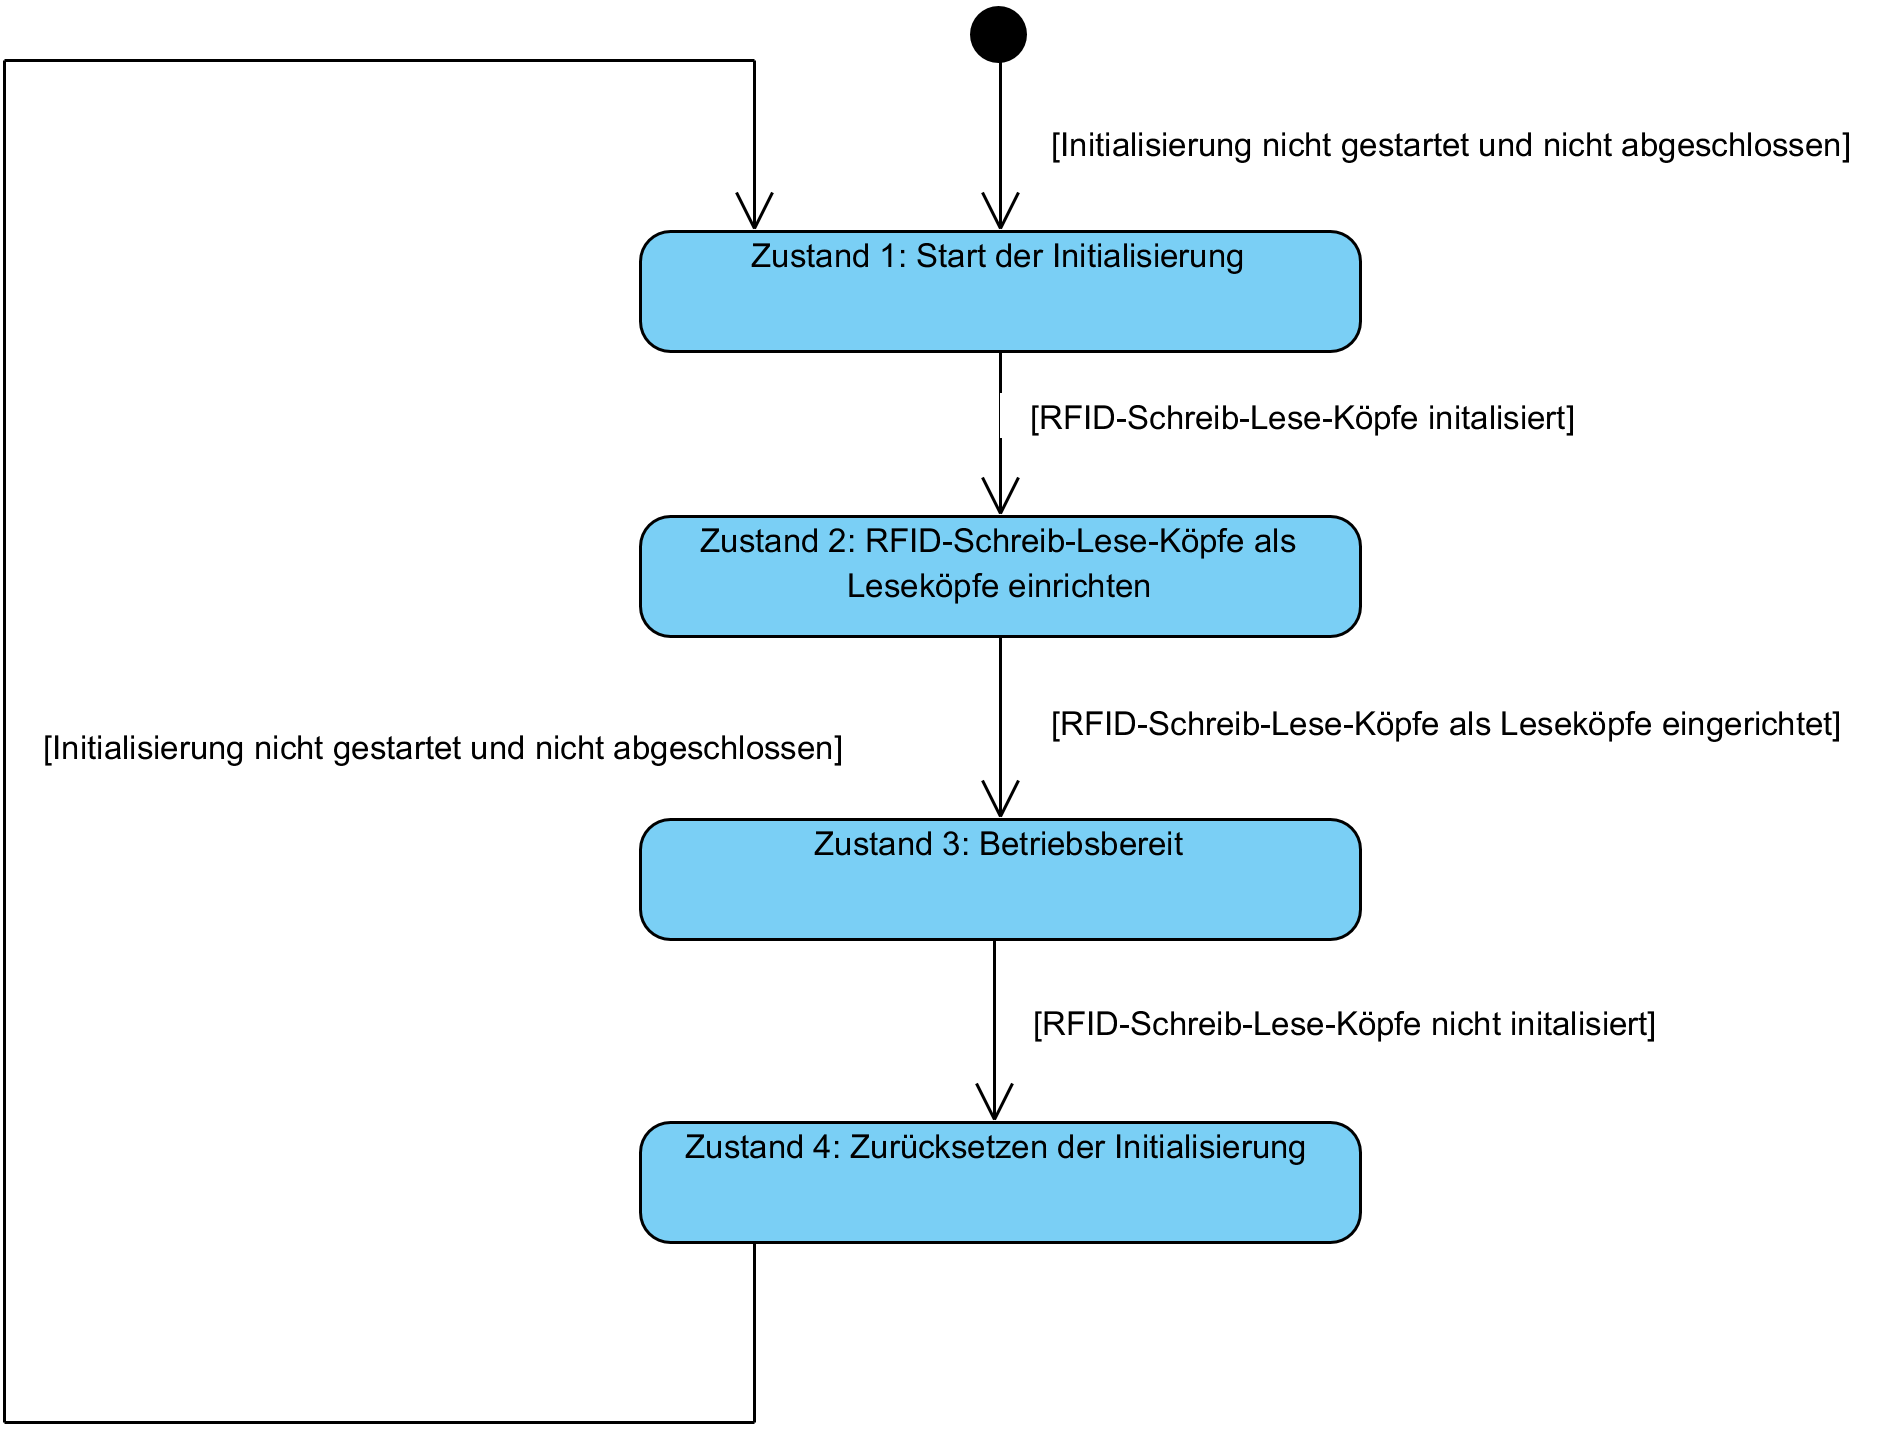
\includegraphics[width=0.7\linewidth]{Bilder/Zustandsdiagramme/RFID_lesen.png}
        \caption{UML-Zustandsdiagramm der Initialisierung der RFID-Leseköpfe 2 bis 8}
        \label{fig:init_Leseköpfe}
\end{figure}

Ist die Initialisierung abgeschlossen, werden die RFID-Schreib-Lese-Köpfe kontinuierlich ausgelesen. Ist ein RFID-Tag unter dem Lesegerät, wird der Wert des Tags in einem Array gespeichert. Dabei entspricht die Stelle im Array der Station, an der der Tag eingelesen wurde. Ist kein Werkstück unter dem Schreib-Lese-Kopf wird in das Array eine 0 geschrieben. Da der Wert, den die Schreib-Lese-Kopf zurück liefern, immer dem des zuletzt eingelesenen RFID-Tags entspricht, wird mithilfe des Parameters TFR überprüft, ob sich aktuell ein RFID-Tag unter dem Schreib-Lese-Kopf befindet. Der TFR-Parameter gibt an, ob sich ein RFID-Tag innerhalb des Lesebereichs befindet. Befindet sich kein RFDI-Tag unter dem Schreib-Lese-Kopf wird der Wert auf 0 gesetzt. Befindet sich ein RFID-Tag darunter wird gewartet bis der RFID-Tag ausgelesen und der Wert ins Array geschrieben wurde. 

Die Informationen werden auf den RFID-Tags als Bytes gespeichert. Zur weiteren Verarbeitung werden die Bytes in einem Integer zusammengefasst. Dies übernimmt die selbst geschriebene Funktion ByteToInt(), die als Eingangsvariable ein Byte-Array und als Ausgangsvariable eine Integervariable hat.

\subsection{FB Aufruf\_RFID\_Channel\_1\_Schreiben}\label{kap:FB_schreiben}
Dieser Funktionsbaustein organisiert das Beschreiben der RFID-Tags an Station 1. Im Aufbau ist er dem in Abschnitt \ref{kap:FB_Lesen} beschriebenen Funktionsbaustein ähnlich. Allerdings befindet sich hier nur eine Instanz des Funktionsbausteins "`FB\_RFID\_SS15"'für den Schreib-Lese-Kopf an Station 1. Der Zustandsautomat entspricht dem in Abbildung \ref{fig:init_Leseköpfe}. Lediglich der Zustand 2 unterscheidet sich, da dort der Schreib-Lese-Kopf nicht als Lesekopf sondern als Schreibkopf eingerichtet wird. 

Über die Rückgabewerte Busy und Done wird detektiert, ob gerade ein RFID-Tag neu beschrieben wurde. Wird ein Schreibvorgang erkannt, wird die Globale-Variable "`WRITE\_RFDI\_DONE"'gesetzt. Diese Variable wird im Funktionsbaustein "`Time\-sta\-mp\_an\-legen"'aus Abschnitt \ref{kap:FB_Timestamp} beim Suchen nach einem neuen Werkstück verwendet. Dort wird sie auch zurückgesetzt. Damit sie nach dem Zurücksetzen nicht sofort wieder gesetzt wird, sollte sich das Werkstück noch unter dem Schreibkopf befinden, wird mittels eines Timers \SI{6}{\second} gewartet. Das bedeutet, dass auch nur alle  \SI{6}{\second} ein Werkstück aus dem Lager geholt werden kann. Die Roboter sind allerdings nicht in der Lage innerhalb von \SI{6}{\second} zwei Werkstücke aus dem Lager zu holen, so dass es zu keinen Problemen führt.

\subsection{FB FB\_RFID\_SS15}
Der Funktionsbaustein"`FB\_RFID\_SS15"'wurde mit dem Starterkit zur Verfügung gestellt. Der im Programm verwendete Funktionsbaustein entspricht fast komplett dem Funktionsbaustein aus dem Starterkit, weshalb er hier nicht weiter erläutert wird. Nur für das Errorhandling sind wenige Zeilen Code hinzugekommen. 

Ist der Rückgabewert "`Channel\_X\_ERROR"'  True wird ein Reset durchgeführt bis der der Fehler behoben wurde. Zum Testen der Fehleranfälligkeit befindet sich ein Zähler im Errorhandling. 

\subsection{FB Werkstueck\_Tagen}\label{kap:FB_werkstueck_taggen}
Immer wenn ein Roboter ein Werkstück aus dem Lager holen soll, wird von der Fertigungsplanung in die Datenbank geschrieben um welches Werkstück es sich handelt. Dieser Funktionsbaustein fragt durchgehend die Datenbank ab und ermittelt so welches die nächste ID ist die an Station 1 auf den RFID-Tag des Werkstücks geschrieben werden muss. In Abbildung \ref{fig:FB_Werkstueck_taggen} ist das dazugehörige Zustandsdiagramm dargestellt.
\begin{figure}[h]
	    \centering
	    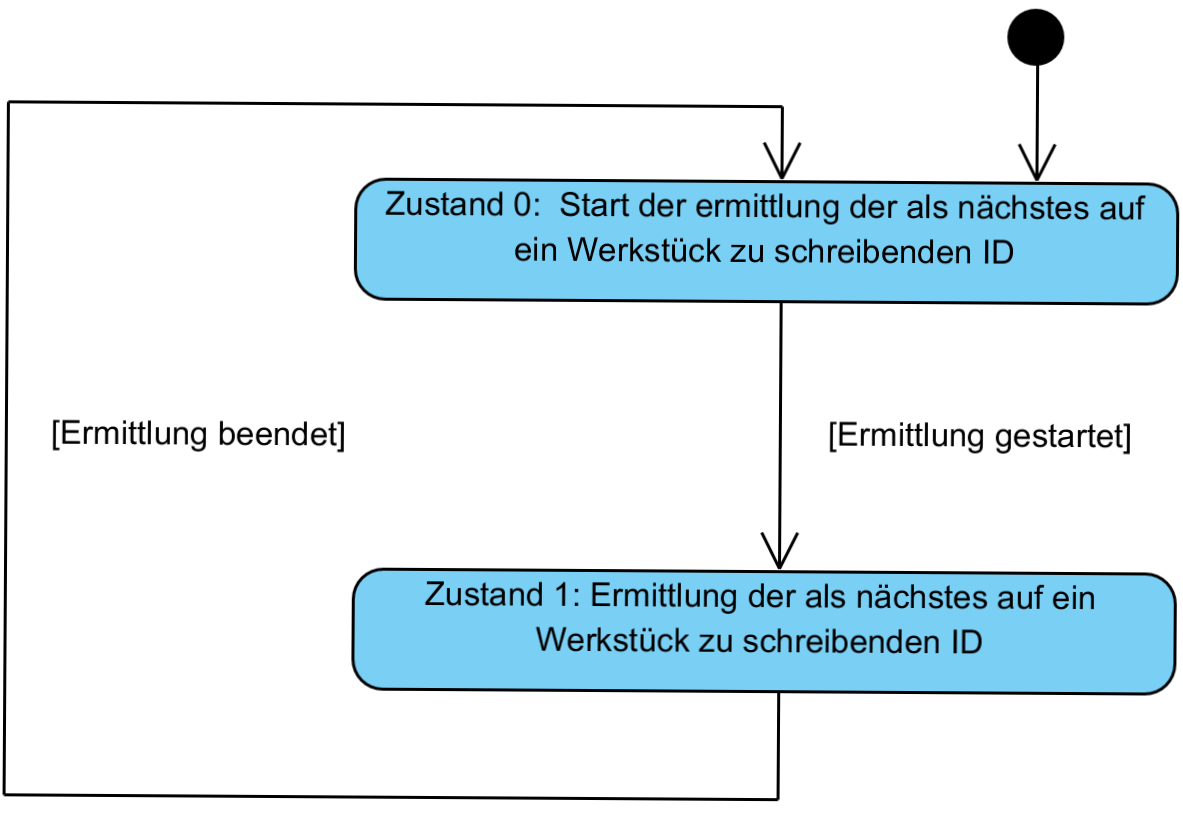
\includegraphics[width=0.7\linewidth]{Bilder/Zustandsdiagramme/taggen.png}
        \caption{UML-Zustandsdiagramm des FB Werkstueck\_taggen}
        \label{fig:FB_Werkstueck_taggen}
\end{figure}

\subsection{FB Timestamp\_anlegen}\label{kap:FB_Timestamp}
Der Funktionsbaustein "`Timestamp\_anlegen"' ist zuständig für die Auswertung des RFID-Arrays, in dem die aktuell eingelesenen Werkstück ID's gespeichert sind. Des Weiteren ermittelt der Funktionsbaustein alle für das Anlegen des Timestamps erforderlichen Werte und schreibt mit Hilfe des Funktionsbausteins "`Datenbank\_Read\_Write"' den Timestamp in die Datenbank. In der Abbildung \ref{fig:FB_Timestamp_anlegen} ist das Zustandsdiagramm des Funktionsbaustein dargestellt. 

\begin{figure}[h]
	    \centering
	    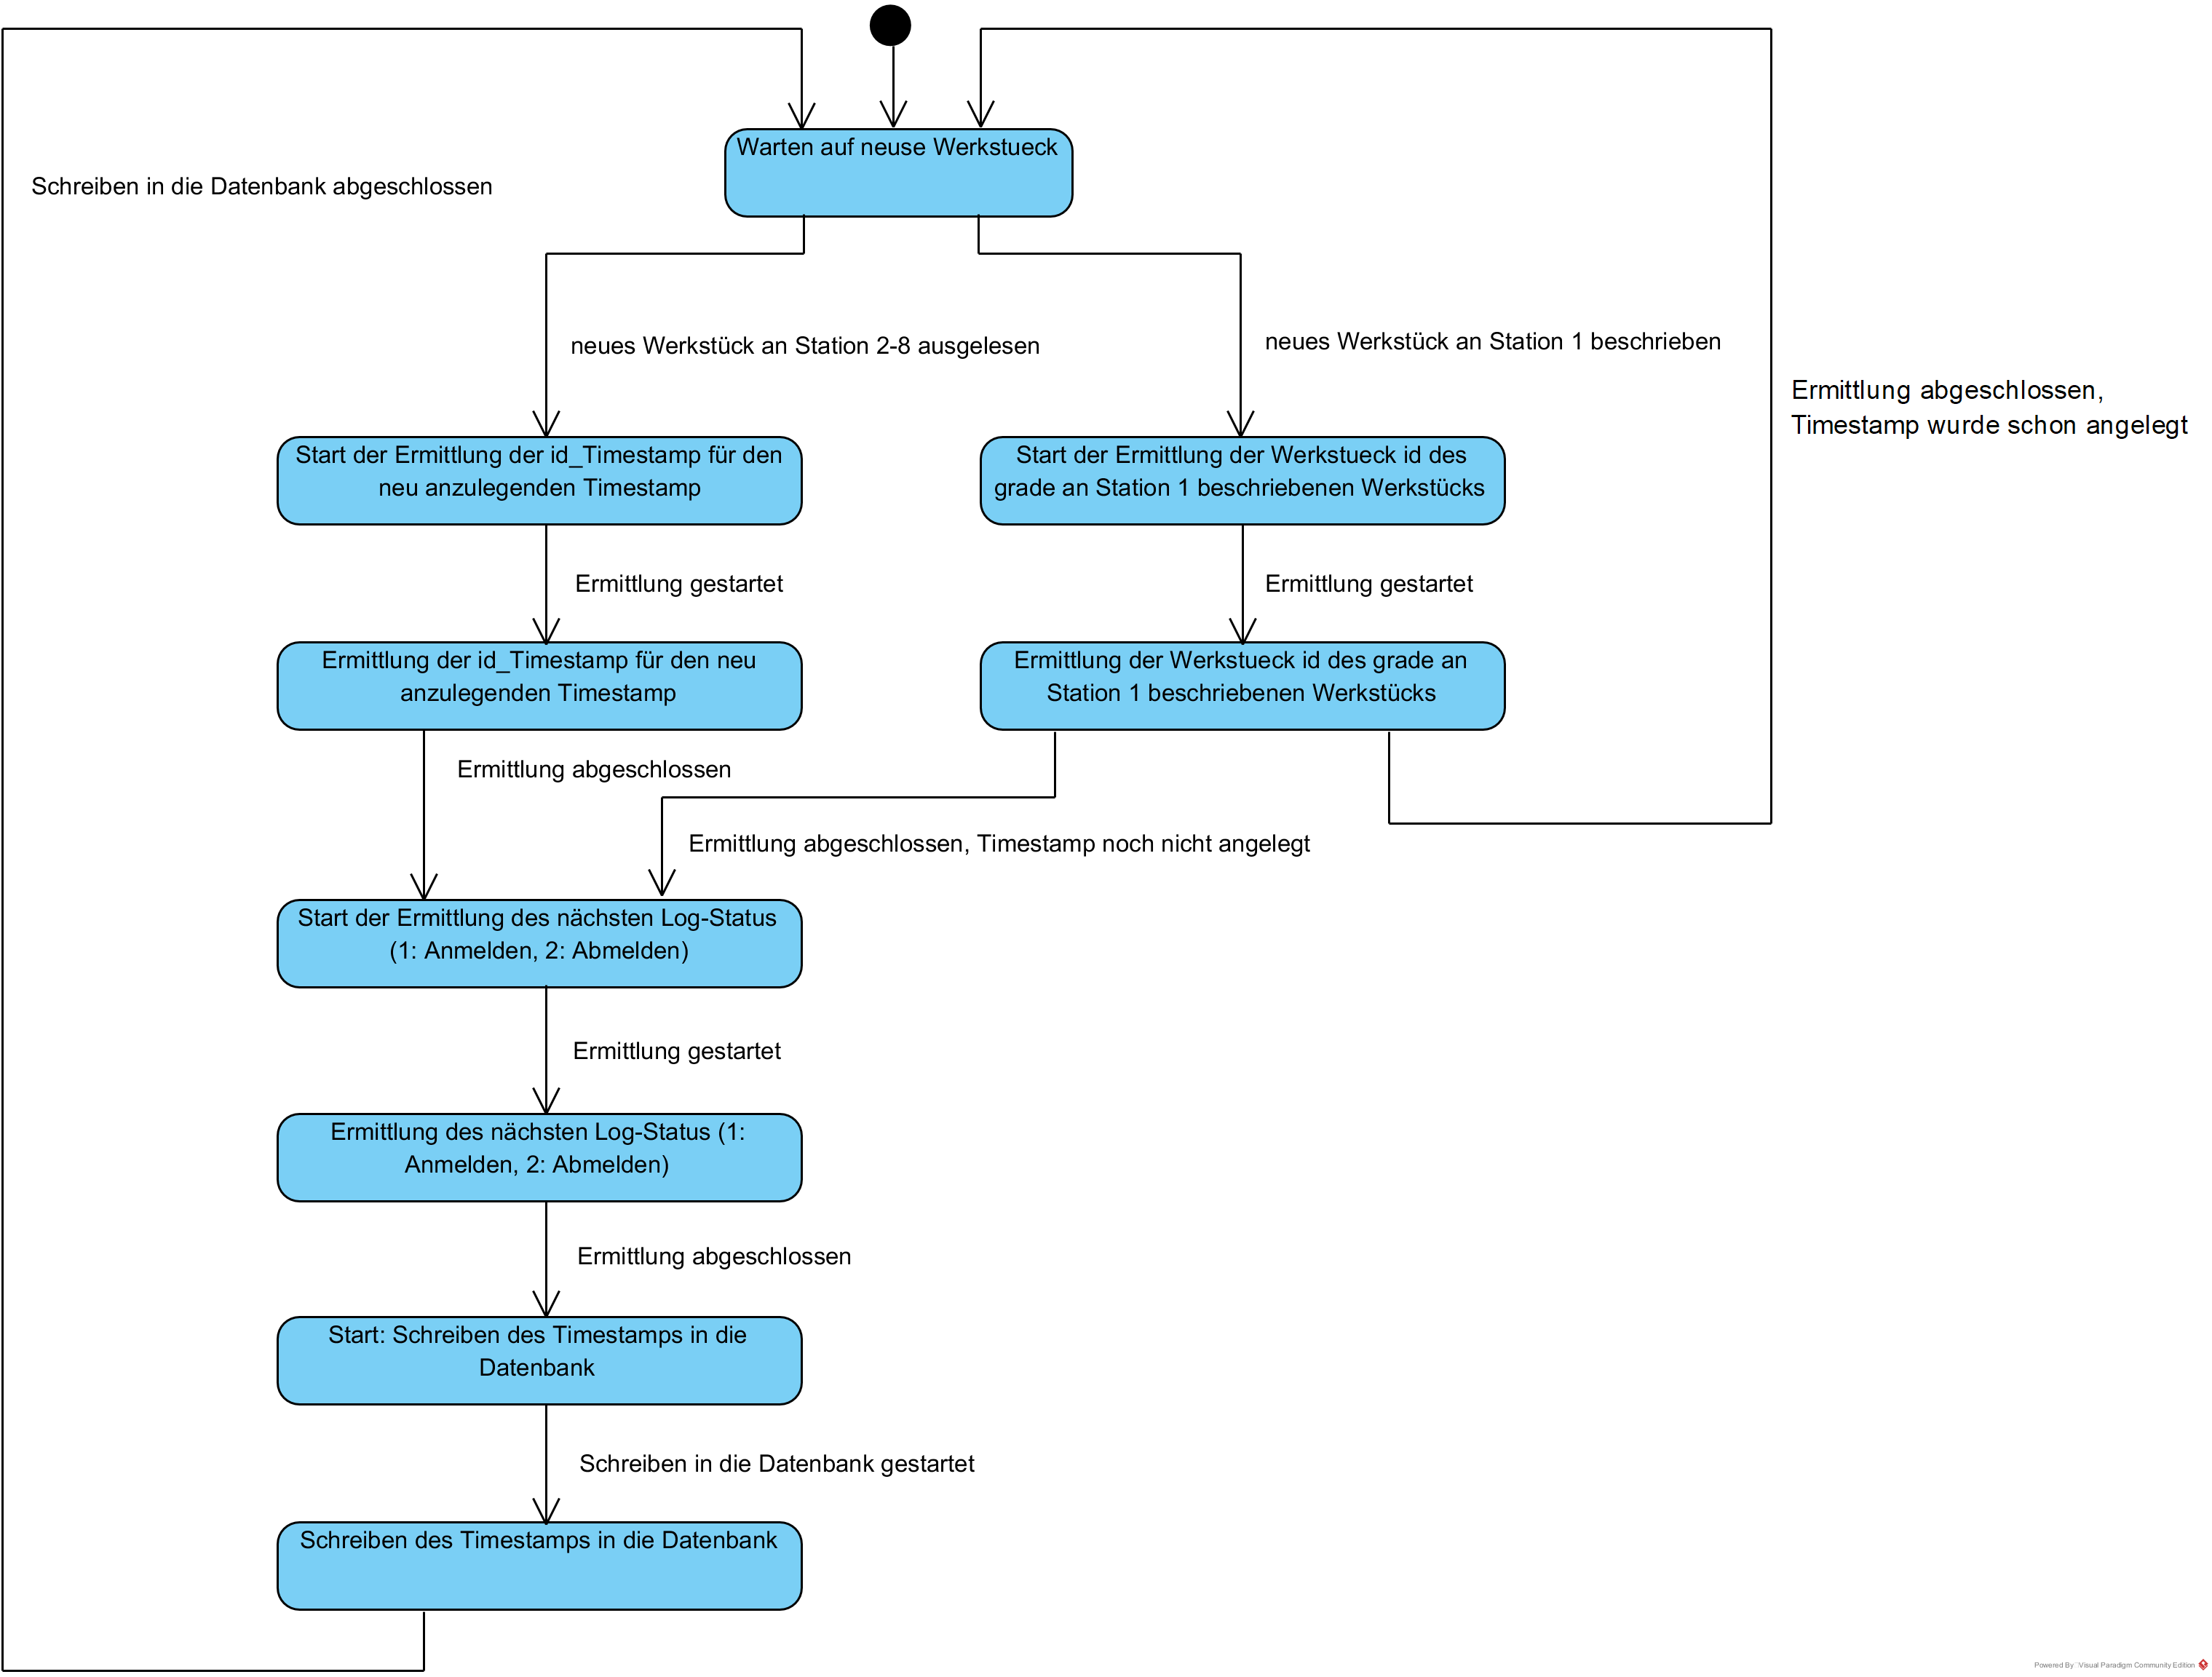
\includegraphics[width=1\linewidth]{Bilder/Zustandsdiagramme/Zustandsautomat_Timestamp.png}
        \caption{UML-Zustandsdiagramm des FB Timestamp\textunderscore anlegen}
        \label{fig:FB_Timestamp_anlegen}
\end{figure}

Zunächst wird im  Zustand 0 mit Hilfe der Funktion "`Suche\textunderscore neues\textunderscore Werkstueck"' nach einem neu unter den RFID-Schreib-Lesekopf geschobenes Werkstück gesucht. Zu Beginn wird allerdings zunächst geprüft, ob an Station 1 ein Werkstück neue beschrieben wurde. Dazu wird die globale Variable "`WRITE\textunderscore RFID\textunderscore DONE"' ausgewertet und ggf. zurückgesetzt. Wurde kein Werkstück neu beschrieben, wird überprüft, ob sich seit dem letzten Aufruf der Funktion ein Wert im RFID-Array geändert hat. Dazu wird ein Vergleich mit einer Kopie des Arrays aus dem letzten Aufruf durchgeführt. Wird eine Änderung erkannt und es handelt sich nicht um eine Änderung auf den Wert 0, wird die Station an der die Änderung aufgetreten ist und die ID des erkannten Werkstücks von der Funktion zurückgegeben. Ebenso wird die geänderte  Kopie des RFID-Arrays zurückgegeben.

Wurde ein Werkstück an Station 1 neu beschrieben, so muss zunächst mit einer Datenbankabfrage aus der Tabelle "`taggen"' die ID des beschriebenen Werkstücks ermittelt werden. Dies geschieht im Zustand 2. Der Zustand 1 startet die Ermittlung. Für einen Zugriff auf die Datenbank werden immer zwei Zustände benötigt, einer in dem signalisiert wird das eine Abfrage stattfinden soll. Beginnt die Abfrage, wird dieser Zustand verlassen und im darauf folgenden Zustand wird gewartet bis die Abfrage abgeschlossen ist. Diese zwei Zustände ergeben sich aus dem Zusammenspiel mit dem global instanziierten Funktionsbaustein "´Datenbank\textunderscore Read\textunderscore Write"', der in Abschnitt \ref{kap:FB_Datenbank_Read_Write} näher beschrieben ist.

Wurde die ID des neu beschriebenen Werkstücks ermittelt, liegen genau die gleichen Informationen, nämlich die ID des Werkstücks und die Station an der es erkannt wurde, wie bei einem Werkstück, dass neu unter einen Lesekopf der Stationen 2-8 geschoben wurde, vor. Für beide möglichen Fälle geht es weiter mit Zustand 3 und 4, in denen die nächste ID für den Timestamp aus der Datenbank ermittelt wird. Beim Übergang von Zustand 4 in Zustand 5 wird die aktuelle Zeit als Unix-Timestamp gespeichert. Anschließend wird im Zustand 5 und 6 der nächste Log-Status ermittelt. Der Log-Status beschreibt, ob es sich um eine Anmeldung oder eine Abmeldung handelt. Zum Ermitteln des Log-Status wird der letzte Eintrag für das jeweilige Werkstück in der Tabelle "`Timestamp"' in der Datenbank ermittelt und der Status dementsprechend gesetzt. Besonders werden die Fälle an Station 1 und an Station 8 behandelt, da dort nur An- beziehungsweise Abmeldungen möglich sind.

Nachdem nun die ID des Werkstücks, die Station, die ID des nächsten Timestamps, der nächste Log-Status und die aktuelle Zeit bekannt sind, werden die Daten in den Zuständen 7 und 8 als Timestamp in der Datenbank abgelegt und zu Zustand 0 zurückgekehrt.

\subsection{FB Datenbank\_Read\_Write}\label{kap:FB_Datenbank_Read_Write}
Der Funktionsbaustein "`Datenbank\_Read\_Write"' sorgt für einen geordneten Zugriff auf die Datenbank. Der eigentliche Zugriff auf die Datenbank findet in den vier Funktionsbausteinen "`SQL4Automation\_id\_Lesen"', "`SQL4Auto\-mation\-\_\-next\-Log\-Sta\-tus\-\_Lesen"', "`SQL\-4Auto\-mat\-ion\_Ti\-me\-stap"' und "`SQL4Auto\-mation\-\_\-RFID\-\_Werkstueck\_Lesen"' statt. Da die Funktionsbausteine die selben globalen Variablen nutzen und mehrere Zyklen für einen Zugriff benötigen, dürfen nicht mehrere der Funktionsbausteine gleichzeitig versuchen auf die Datenbank zuzugreifen. Weil aber Anfragen an die Datenbank von zwei verschiedenen Funktionsbausteinen aus erfolgen, muss sichergestellt sein, dass diese Anfragen nicht gleichzeitig erfolgen. Dafür wird dieser global instanziierte Funktionsbaustein genutzt. Wenn aus einem der lokal instanziierten Funktionsbausteine heraus eine Anfrage gestellt wird, prüft der Funktionsbaustein "`Datenbank\_Read\_Write"', ob diese Anfrage gerade möglich ist. Sollte die Anfrage nicht an der Reihe sein, wartet der Funktionsbaustein der die Anfrage gestellt hat, bis der Funktionsbaustein "`Datenbank\_Read\_Write"' die Anfrage zulässt und die Abfrage der Datenbank startet. 

Der Funktionsbaustein "`Datenbank\_Read\_Write"' prüft in dem Zustandsautomaten aus Abbildung \ref{fig:FB_Datenbank_Read_Write}, ob eine Anfrage für den jeweiligen Datenbankzugriff vorliegt. Liegt keine Anfrage vor, geht er zum nächsten Zustand, in dem auf eine Anfrage geprüft wird. Liegt einen Anfrage vor startet er einen Datenbankzugriff und geht für die Dauer des Zugriffs in einen Zustand, der die Anfrage ausführt. An die anfragenden Funktionsbausteine meldet er zurück. ob ein Datenbankzugriff gestartet wurde und ob der gestartete Zugriff abgeschlossen wurde.  Während sich der Funktionsbaustein in einem ausführenden Zustand befindet, werden weiter Anfrage der anderen Funktionsbausteine abgelehnt.
\begin{figure}[!htb]
	    \centering
	    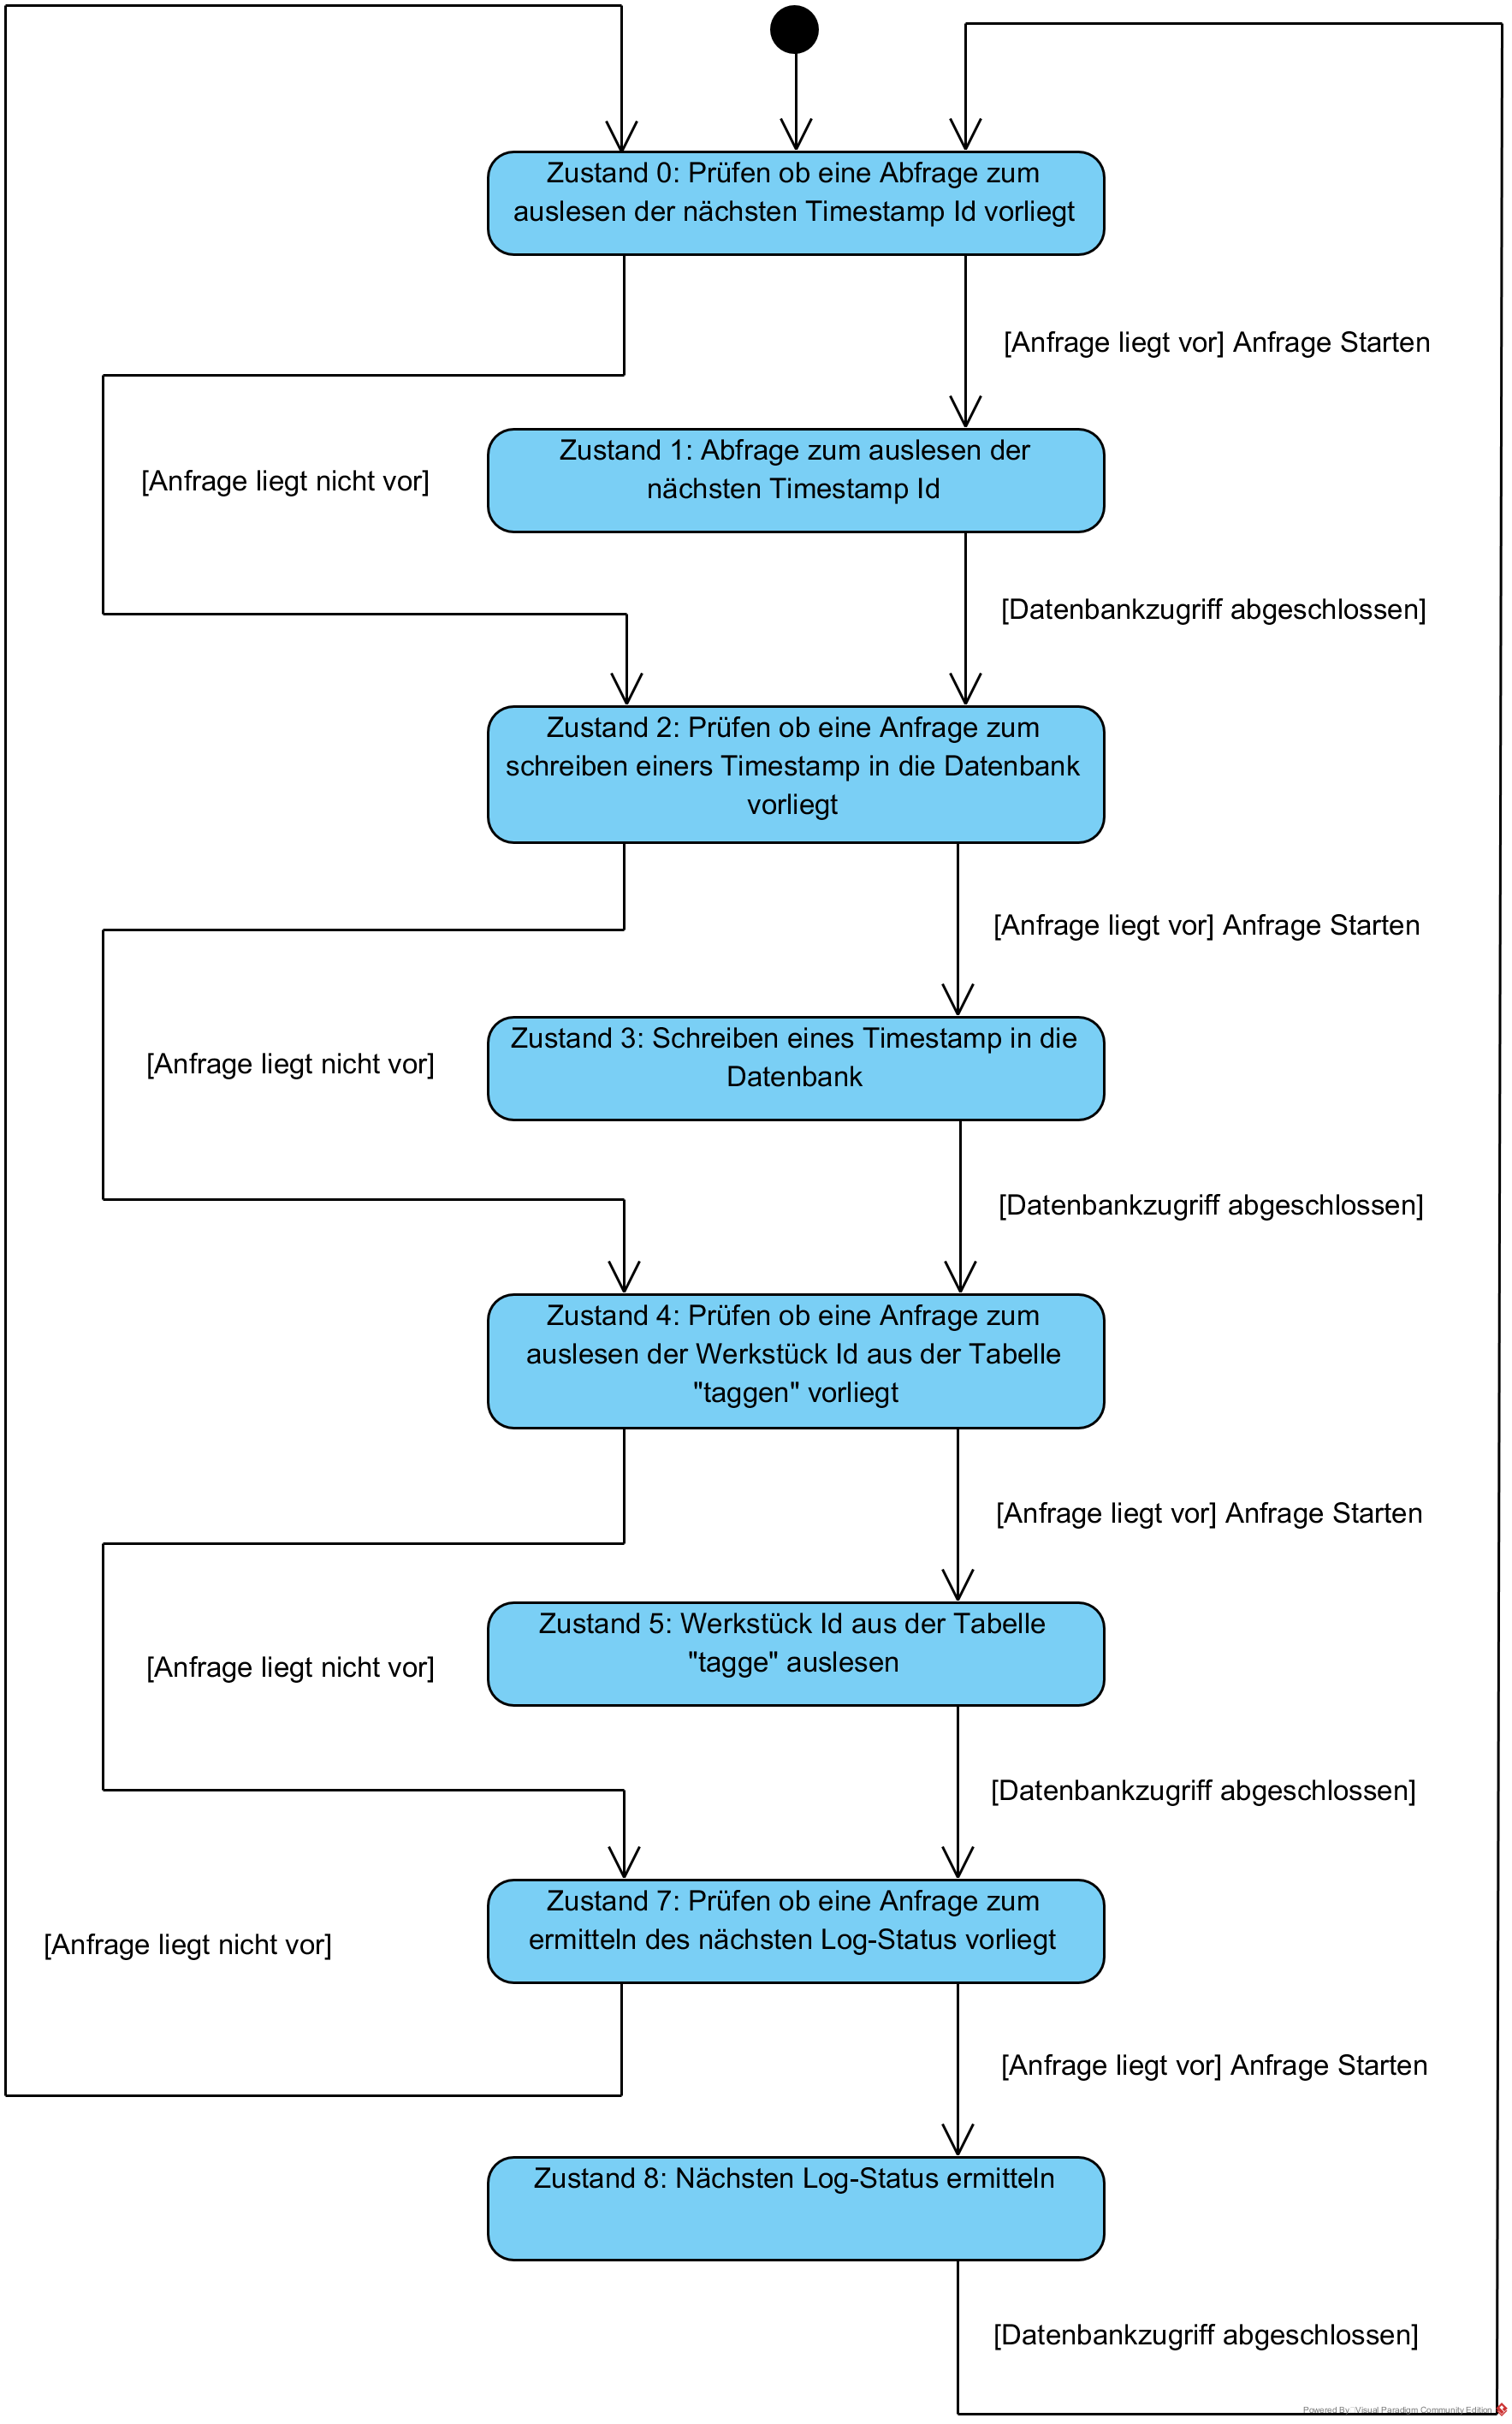
\includegraphics[width=0.8\linewidth]{Bilder/Zustandsdiagramme/Datenbank_Read_Write_State_Machine_Diagram.png}
        \caption{UML-Zustandsdiagramm des FB Datenbank\_Read\_Write}
        \label{fig:FB_Datenbank_Read_Write}
\end{figure}

\subsection{FB SQL4Automation}\label{kap:FB_SQL4Automation}
Für jeden Zugriff auf die Datenbank ist ein separater Funktionsbaustein zuständig. Aufgerufen werden die Funktionsbausteine durch den global instanziierten Funktionsbaustein "`Daten\-ba\-nk\_Read\_Write"', der in Abschnitt \ref{kap:FB_Datenbank_Read_Write} beschrieben ist. Die Funktionsbausteine entsprechen in großen Teilen dem mit dem Staterkit zur Verfügung gestellten Funktionsbaustein "`SQL4Auto\-mat\-ion\_2015"'. Angepasst wurde für die jeweiligen Funktionsbausteine der MySQL-Befehl zum Lesen oder Schreiben in der Datenbank. Des Weiteren wurde bei Lesebefehlen ein zusätzlicher Rückgabewert für das Ergebnis der Abfrage und die entsprechende Konvertierung des Rückgabe-Strings der Datenbank in den richtigen Datentyp hinzugefügt. Ebenso wurde eine Rückgabevariable hinzugefügt, die zurückmeldet, ob die Anfrage an die Datenbank abgeschlossen ist. Wie schon in Kapitel \ref{kap:FB_Datenbank_Read_Write} beschrieben, nutzen alle Funktionsbausteine, die den Zugriff auf die Datenbank durchführen, die selben globalen Variablen. Da ein Zugriff mehrere Zyklen dauert, ist sicherzustellen, dass nicht zwei Funktionsbausteine zur selben Zeit eine Anfrage an die Datenbank stellen. 



\subsection{Einstellen der Systemzeit}
\label{kap:Systemzeit_Einstellen}
Da die Systemzeit nach jedem Start der Soft-SPS auf den default-Wert 1. Januar 1970 0:00:00 Uhr gesetzt wird und das manuelle Einstellen der Systemzeit bei jedem Neustart der Soft-SPS, beziehungsweise des aufgespielten CODESYS-Programms, ungenau und aufwendig ist, wird die aktuelle mitteleuropäische Zeit zu Beginn des Programms automatisch ermittelt. Zur Ermittlung der Zeit für die Timestamps wird der Funktionsbaustein "`RTC"' genutzt. Dieser wird zu Programmbegin im Funktionsbaustein "`Timestamp\_anlegen"' einmal initialisiert. Für die Initialisierung wird die aktuelle Zeit im Datentype DT benötigt. Die aktuelle Zeit wird zu Programmbegin in der Main über die Datenbank ermittelt. 

Wie in Abbildung \ref{fig:ER-Diagramm_Worbenche} zu sehen, gibt es in der Datenbank eine Tabelle mit dem Namen Zeit, diese Tabelle hat nur eine Zeile in der es einmal den Primärschlüssel "`id\_Zeit"' und das Feld "`aktuelle\_Zeit"' gibt. Bei Start des Programms wird in der Main zunächst der Funktionsbaustein "`SQL4Automation\_aktuelle\_Zeit"' aufgerufen. Dabei handelt es sich um den einzigen Funktionsbaustein der auf die Datenbank zugreift und nicht über den Funktionsbaustein "`Datenbank\_Read\_Write"' aufgerufen wird. Da das Ermitteln der aktuellen Zeit erst abgeschlossen sein muss, bevor der restliche Programmteil startet, besteht keine Gefahr eines gleichzeitigen Zugriffs.
Der Funktionsbaustein "`SQL4Automation\_aktuelle\_Zeit"' führt die zwei in den Listings \ref{lst:MySQL_Zeit1} und \ref{lst:MySQL_Zeit2} dokumentierten SQL-Befehle aus.
Der Befehl aus Listing \ref{lst:MySQL_Zeit1} aktualisiert die Zeit im Feld "`aktuelle\_Zeit"' in der Datenbank. Dazu wird ein Update der einzigen Zeile in der Tabelle ausgeführt. Besonders ist hierbei der SET-Befehl, der dem Feld "`aktuelle\_Zeit"' den Rückgabewert der MySQL-Funktion NOW() zuweist (Zeile 3). Die Funktion NOW() liefert die aktuelle Zeit, abhängig von der konfigurierten Zeitzone. Mit dem Befehl in Listing \ref{lst:MySQL_Zeit2} wird diese abgefragt.
\lstset{ 
    keywordstyle        =\bfseries\ttfamily\color{blue},
    basicstyle          =\scriptsize\ttfamily, 
    emphstyle           =\color{red},
    numbers             =left,
    xleftmargin         =15pt,
    backgroundcolor     =\color{newgray},
    showstringspaces    =false,
    language            =SQL
    }	 

\begin{lstlisting}[caption={MySQL-Befehl: Zeit aktualisieren}
       \label{lst:MySQL_Zeit1},
       captionpos=t] 
UPDATE vpj.Zeit
SET
    aktuelle_Zeit = NOW()
WHERE
    id_ZEIT = 1;
\end{lstlisting}

\lstset{ 
    keywordstyle        =\bfseries\ttfamily\color{blue},
    basicstyle          =\scriptsize\ttfamily, 
    emphstyle           =\color{red},
    numbers             =left,
    xleftmargin         =15pt,
    backgroundcolor     =\color{newgray},
    showstringspaces    =false,
    language            =SQL
    }	 

\begin{lstlisting}[caption={MySQL-Befehl: Zeit abfragen}
       \label{lst:MySQL_Zeit2},
       captionpos=t] 
SELECT
    aktuelle_Zeit
FROM
    vpj.Zeit
WHERE
    id_ZEIT = 1;
\end{lstlisting}

Mit Hilfe von String-Operationen wird der zurückgelieferte String so umgebaut, dass er mit Hilfe eines Cast vom Datentyp String in den Datentyp DT (Date and Time) umgewandelt werden kann. Ist die Ermittlung der aktuellen Zeit abgeschlossen, startet das eigentliche Programm.